\section{Numerical analysis and errors}

Numerical analysis is the branch of mathematics concerned with employing electronic calculators to discover solutions for specific mathematical problems. 
It represents the fusion of mathematical principles and computer science.
On the other hand, scientific computing also involves the formalization of models, requiring a foundation in engineering knowledge.
\begin{figure}[H]
    \centering
    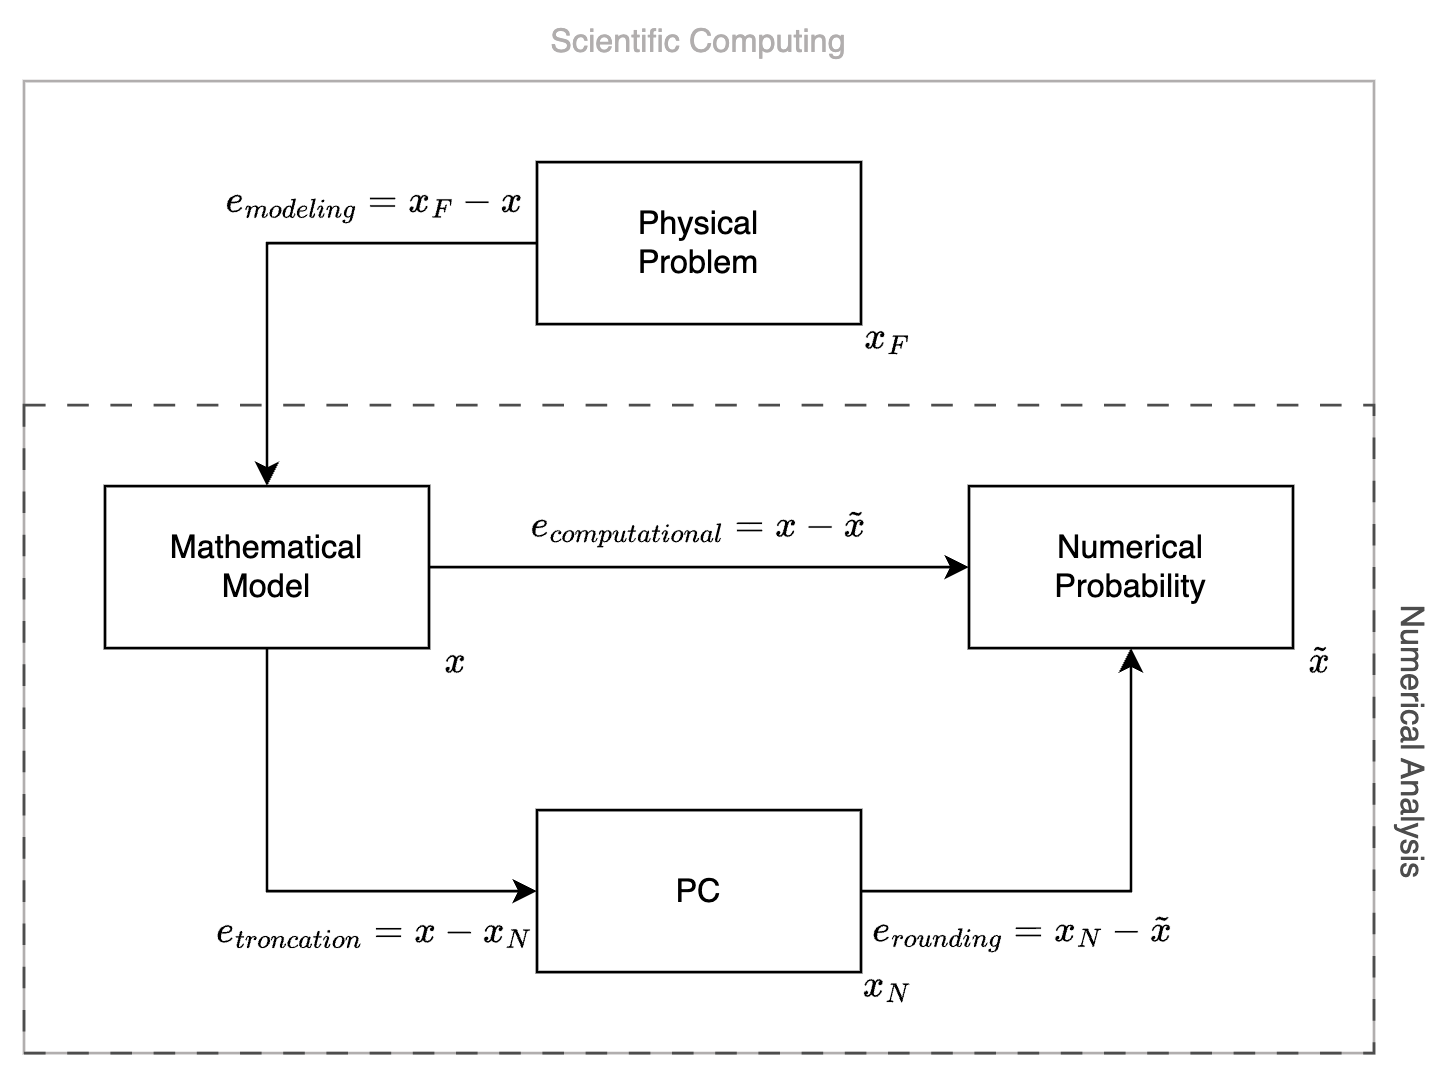
\includegraphics[width=0.75\linewidth]{images/difference.png}
    \caption{Difference between numerical analysis and scientific computing}
\end{figure}
As evident in the diagram, each computational step encounters errors. These errors can be categorized into two types:
\begin{itemize}
    \item Absolute: $\left\lvert x - \tilde{x} \right\rvert$
    \item Relative: $\dfrac{\left\lvert x - \tilde{x} \right\rvert}{\left\lvert x \right\rvert}$, where $x \neq 0$
\end{itemize}
The relative error is considered more precise as it relates the error to the measured quantity.
\begin{example}
    Let's take $x=100$ and $\tilde{x}=100.1$. 
    In this case, the errors are as follows:
    \[e_{abs}=\left\lvert x - \tilde{x} \right\rvert=\left\lvert 100 - 100.1 \right\rvert=0.1\]
    \[e_{rel}=\dfrac{\left\lvert x - \tilde{x} \right\rvert}{\left\lvert x \right\rvert}=\dfrac{\left\lvert 100 - 100.1 \right\rvert}{\left\lvert 100 \right\rvert}=0.001\]
    Now, consider $x=0.2$ and $\tilde{x}=0.1$. 
    In this case, the errors are as follows:
    \[e_{abs}=\left\lvert x - \tilde{x} \right\rvert=\left\lvert 0.2 - 0.1 \right\rvert=0.1\]
    \[e_{rel}=\dfrac{\left\lvert x - \tilde{x} \right\rvert}{\left\lvert x \right\rvert}=\dfrac{\left\lvert 0.2 - 0.1 \right\rvert}{\left\lvert 0.2 \right\rvert}=0.5\]
    The results show that in both examples, the absolute error is the same (0.1), which represents a $10\%$ error. 
    However, the relative error differs significantly.
    In the second example, the relative error is $50\%$, while in the first example, it is only $0.1\%$. 
\end{example}